\section{Adatbázisséma}

\subsection{Tervezés}

Az adatbázisséma tervezéséhez a dbdiagram.io nevű platformfüggetlen, webes ER diagram tervező szoftvert használtam.
Ez egy saját fejlesztésű, DBML nevű DSL nyelvet használ a séma leírására, és lehetővé teszi ennek exportálását különféle formátumokba.

\begin{figure}[!ht]
\centering
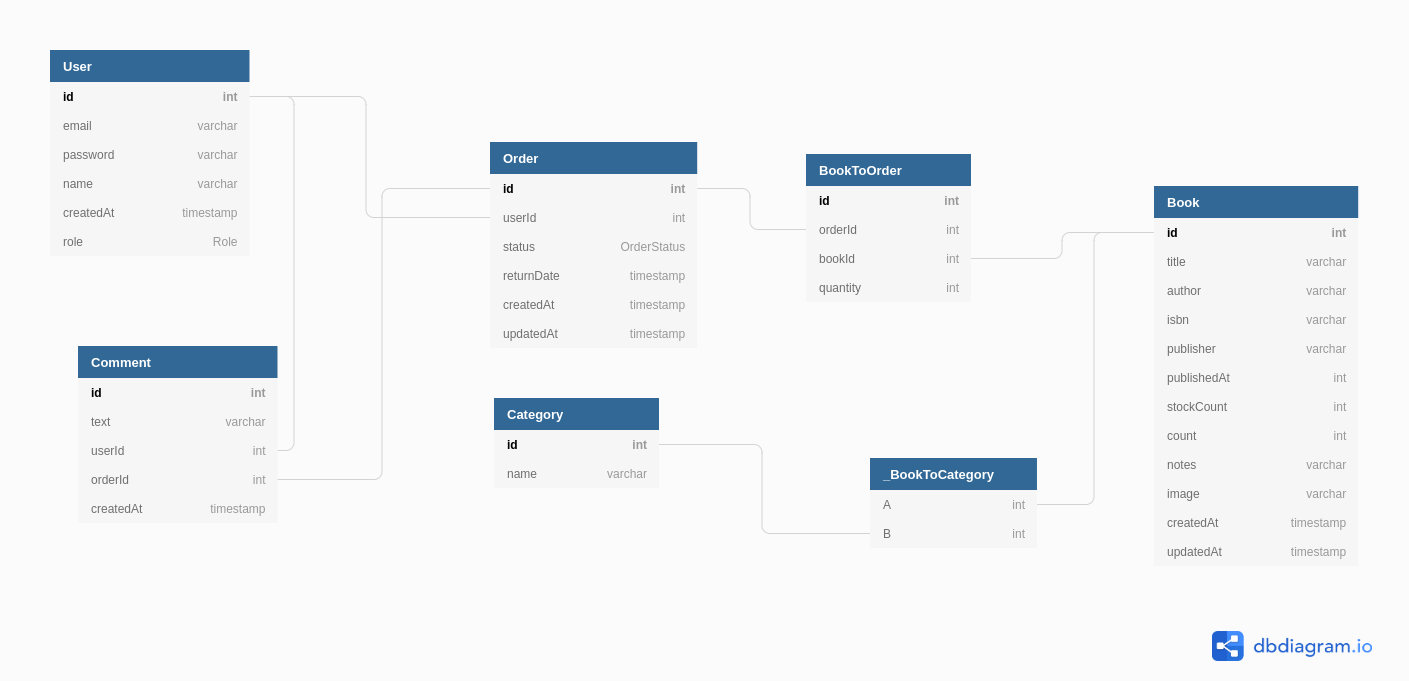
\includegraphics[width=150mm, keepaspectratio]{figures/dbschema.png}
\caption{Az adatbázisséma ER diagramja.}
\label{fig:DBSchema}
\end{figure}

A séma tervezése során a Prisma által használt elnevezési konvenciókat használtam megkönnyítve a két technológia közötti átjárhatóságot.

\subsection{Implementáció}

A séma adatbázisba történő átvezetésére két lehetőségünk van. Az egyik, hogy a dbdiagram oldalról lehetőségünk van .sql kiterjesztésű fájlt letölteni,
ezt a létrehozott adatbázisunkon futtatni, majd a Prisma introspect funkcióját használva legenerálni hozzá a Prisma schema fájlt a backendünk számára.
A másik, egyszerűbb megoldás a Prisma migrate\footnote{A dolgozat írása idejében ez a funkció még experimental státuszban volt, de a használata során nem ütköztem problémákba.} használata.
Ez esetben nekünk manuálisan kell létrehozni a Prisma schema fájlt a korábbi diagram alapján, majd a
\begin{lstlisting}
prisma migrate save --experimental
prisma migrate up --experimental
\end{lstlisting}

parancsokat kiadva létrehozzuk és futtatjuk a Prisma migrációt.
Ez utóbbi megoldás előnyei, hogy egy központi helyen tudjuk kezelni a séma változásait, valamint ezt adatbázis-agnosztikus módon
tehetjük meg.

A Prisma DSL-ben a dbdiagram.io-hoz hasonló módon tudjuk felvenni a relációkat. Ennek nagy előnye, hogy a táblák közötti kapcsolatokat
egyszerűen tudjuk modellezni, amit a \lstinline|prisma migrate| át tud vezetni az adatbázisunkba.

\begin{lstlisting}[caption=Séma leírása a Prisma DSL-ben]
generator client {
  provider = "prisma-client-js"
}

datasource db {
  provider = "postgresql"
  url      = env("DATABASE_URL")
}

model Book {
  id          Int           @id @default(autoincrement())
  title       String
  author      String?
  isbn        String?
  publisher   String?
  publishedAt Int?
  stockCount  Int?          @default(1)
  count       Int?          @default(1)
  notes       String?
  image       String?
  createdAt   DateTime?     @default(now())
  updatedAt   DateTime?     @default(now())
  orders      BookToOrder[]
  categories  Category[]
}

model BookToOrder {
  id       Int   @id @default(autoincrement())
  orderId  Int
  bookId   Int
  quantity Int?  @default(1)
  books    Book  @relation(fields: [bookId], references: [id])
  orders   Order @relation(fields: [orderId], references: [id])

  @@unique([bookId, orderId], name: "BookToOrder_book_order_unique")
}

model Category {
  id    Int    @id @default(autoincrement())
  name  String
  books Book[]
}

model Comment {
  id        Int       @id @default(autoincrement())
  text      String?
  createdAt DateTime? @default(now())
  userId    Int
  orderId   Int
  order     Order     @relation(fields: [orderId], references: [id])
  user      User      @relation(fields: [userId], references: [id])
}

model Order {
  id         Int           @id @default(autoincrement())
  userId     Int
  returnDate DateTime?
  status     orderstatus?  @default(PENDING)
  createdAt  DateTime?     @default(now())
  updatedAt  DateTime?     @default(now())
  user       User          @relation(fields: [userId], references: [id])
  books      BookToOrder[]
  comments   Comment[]
}

model User {
  id        Int       @id @default(autoincrement())
  email     String    @unique
  password  String
  name      String?
  createdAt DateTime? @default(now())
  role      userrole? @default(BASIC)
  comments  Comment[]
  orders    Order[]
}

enum orderstatus {
  PENDING
  RENTED
  RETURNED
  LATE
}

enum userrole {
  BASIC
  ADMIN
  EDITOR
}
\end{lstlisting}

